\documentclass[10pt,a4paper,twocolumn,DIV18]{scrartcl}   

\PassOptionsToPackage{hyphens}{url}\usepackage[linktocpage,bookmarks]{hyperref}
\hypersetup{    pdfauthor={Name des Authors},
                pdftitle={Titel},
                pdfsubject={},
                colorlinks=true,
                citecolor=black,
                linkcolor=black,
                urlcolor=black}
\usepackage[latin1]{inputenc}
\usepackage[T1]{fontenc}
\usepackage{bbm}
\usepackage{ae,aecompl}
\usepackage{subfigure}
\usepackage{graphicx}
\usepackage{amsmath}
\usepackage{url}
\usepackage{acronym}
\usepackage[numbers]{natbib}
\usepackage{textcomp}

\pdfstringdefDisableCommands{
	\let\cite\@gobble % remove also first argument
}
\pdfstringdefDisableCommands{
	\let\\\empty % remove also first argument
}
\title{Expos\'e - Deep Learning}
\subtitle{Aerial Cactus Identification}

\author{Wei-Hung Hsu, Tim Schneider, Matthias Heinrich}

\date{April 21th, 2019}

\RedeclareSectionCommand[%
	beforeskip=-0.5\baselineskip
]{paragraph}

\begin{document}  

\maketitle
\begin{abstract}
We implement an Convolutional Neural Network to learn a classifier that detects cacti based on an kaggle challenge\cite{KAGGLE}. 
\end{abstract}
\newcommand{\feat}{\texttt}

%\paragraph*{Abstract}
%\begin{abstract}
%	TODO
%\end{abstract}



%      \begin{figure}[!htb]
%        \center{\includegraphics[width=0.5\textwidth]
%        {images/20190419001057_1.jpg}}
%        \caption{\label{fig1} Player performance, accessable in-game: Number of normal attacks, number of CA, number of CA-Chips, etc.}
%      \end{figure}

%  (fig. \ref{fig1}, \ref{fig2}) 
%  An example is Chitnis et al.\cite{chitnis} 


\section{Motivation}
Object detection or object recognition is one of the most common problem across scientific fields. In the scope of this project we want to implement such a system. Under the pretext of entering the Kaggle competition, Aerial Cactus Identification, we want to study the fundamental practice of convolutional neural network (CNN). The goal of the competition is to assess the impact of climate change on flora and fauna. The sysytem VIGIA, an autonomous surveillance of protected areas, was build for the exact purpose. An important part of such as system is to be able to identify certain vegetation within the protected areas.




\section{Data}
The dataset consists of 17,500 aerial images out of which 13,136 contain an columnar cacti  and 4,364 do not.  Each image is 32x32 in size. The images have been resized by kaggle to be uniform in size. The dataset also contains an .csv file that annoates for each image if it contains an columnar cacti or not. The images are all from the Tehucan-Cuicatlan valley in the south of Mexico.  \cite{LOPEZJIMENZ2019} The images have been obtained using a drone from an flight altitude of 100 m. The images were manually labeled.
      \begin{figure}[!htb]
        \center{
\includegraphics[width=0.5\textwidth]
        {images/test.jpg}}
        \caption{\label{fig1} test \cite{whit}}
      \end{figure}

\section{Data}
The dataset was obtained from kaggle\cite{imet}.
It contains 109,237 images of museum artifacts from the Metropolitan Museum of Art in New York.
The exact source of the images is unknown.
All objects have been labeled by  annotators without verification, thus noisy data is to be expected.
Each annotator was asked to label what he sees in the image.
Labels can describe what culture this object belongs too, or what the object was used for.
For example the image in figure \ref{fig:1} was annotated with: german, nymphenburg, children, female nudes and utilitarian objects.
Figure \ref{fig:2} shows some more example data.
\begin{figure}[h]
    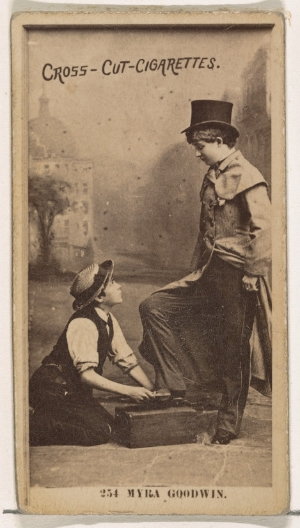
\includegraphics[width=0.5\textwidth]{images/1}
    \caption{A teapot}
    \label{fig:1}
\end{figure}
Furthermore 7,443 images are available for verification.
Both the training and verification image-sets have an corresponding csv-file where one row corresponds with one image.
The images are labeled using numbers, an additional csv-file is given containing the corresponding attributes for each number.
There are 1103 labels in total.
\begin{figure}[h]
    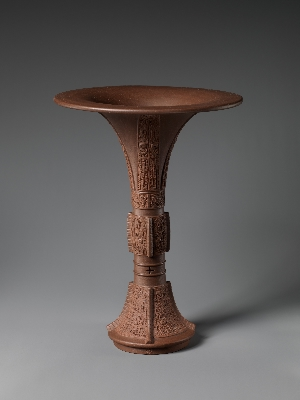
\includegraphics[width=.2\textwidth]{images/3}
    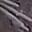
\includegraphics[width=.2\textwidth]{images/4}
    \caption{Example images from the dataset}
    \label{fig:2}
\end{figure}

\section{Implementation}
For implementation we plan to use Python 3.7 with keras\cite{KERAS} and sciPY\cite{SCIPY}, in particular numpy and pandas. 
As an extension of the project we look towards trying out different libraries, such as fast.ai\cite{FASTAI} and compare the different results.
% If we have enough time left at the end of the project we might also try different libraries and compare if we can get better results that way.

\bibliographystyle{plainnat}
\bibliography{bibliography}


\end{document}